\documentclass[a4paper, 11pt, twocolumn]{report}
\usepackage[
	backend=biber,
	natbib=true,
	style=numeric,
	sorting=none
]{biblatex}
\addbibresource{report.bib}
\usepackage{authblk}
\usepackage[left=0.7in, right=0.7in, top=0.7in, bottom=0.9in]{geometry}
\usepackage{listings}
\usepackage{graphicx}
\usepackage{bm}
\usepackage{array}
\usepackage{mathtools}
\usepackage{amssymb}
\usepackage{wrapfig}
\usepackage{listings}
\usepackage{tabulary}
\usepackage{algorithmicx}
\usepackage[font=small,skip=2pt]{caption}
\hyphenpenalty=10000
\linespread{1.03}
\setlength{\columnsep}{0.25in}
\renewcommand{\thesection}{\arabic{section}}

\begin{document}
\lstset{language=Matlab, basicstyle=\small}
\title{\textbf{COMP6208 Advanced Machine Learning} \\
{\Large Student Mini-Projects}}

\author{\textbf{Alexander Ally} (aa2g11)\\
\textbf{Hendrik Appel} (hja1g11)\\
\textbf{Samir Moussa} (sm28g11)}

\affil{School of Electronics and Computer Science\\
Faculty of Physical Sciences and Engineering\\
University of Southampton}
\date{Thursday 7\textsuperscript{th} May 2015}
\maketitle

\begin{abstract}

This is a report describing the preprocessing methods, machine learning algorithms and validation techniques used to find a solution to a typical real-world machine learning problem in the driver telematics analysis space. The task is to model individual drivers based on their driving behaviour specified by their trip data. Several approaches were studied and utilised to find a practical solution to a challenging task and these are explained in this report.

\end{abstract}

% section
\section{Introduction}





% section
\section{Problem Scenario}

\subsection{Dataset}

\subsection{Challenges}

\subsection{Variant Approaches}






% section
\section{Analysis \& Experimentation}

\subsection{Preprocessing}

Forming useful features from unstructured data allows learning algorithms to perform well while minimising the amount of redundant data. A system named \textit{representation learning} requires a model to not only learn a mapping function from input to output, but intrinsically learn a representation of the data within the model. As discussed later, unsupervised learning techniques, particularly deep learning, aim to apply representation learning to establish a expressive representation of the underlying data, enough to extract useful information and reason about new information.

Since the raw data is unstructured and does not provide useful, or in fact any description of the important underlying features surrounding that of a driver and their driving behaviour, much of the complications faced throughout the project arose from the extraction of effective features. The trips were merely composed of sequences of GPS co-ordinates taken at one-second intervals. The data had to be processed and features were to be designed before machine learning techniques could be applied to make predictions. In addition the GPS co-ordinates given in the data were subject to inaccuracy. 

The extracted features contained $N_F$ continuous variables and can be summarised by the following list:

\begin{itemize}
\item Feature 1
\item Feature 2
\end{itemize}


\subsection{Data Smoothing}
Because the features were often based upon first and second order gradients of the original data, noise caused a lot of problems. Particularly when the speed of the vehicle was low, small fluctuations in the position of the vehicle caused a small velocity and acceleration to be reported. When directional information is extracted from these gradients (and magnitude information thrown away) there would appear to be wild changes in direction when really the vehicle was stationary and there was small fluctuations in the position information being reported. 

In order to solve this problem a number of different avenues were explored. One simple approach was report any velocity with a magnitude of less than a small value to be set to 0. However this ignored smoothness issues that occurred at higher speeds. To remedy this a simple filter was constructed by applying the Discrete Fourier Transform and reconstructing th data using fewer components. This does appear to work well in general but in sections where the driver is crawling along at a very low speed were the filter wrongly assumes that the driver is stationary. This can be observed in the plot in figure \ref{fig:fouriersmooth}.

\begin{figure}[h]
    \center
    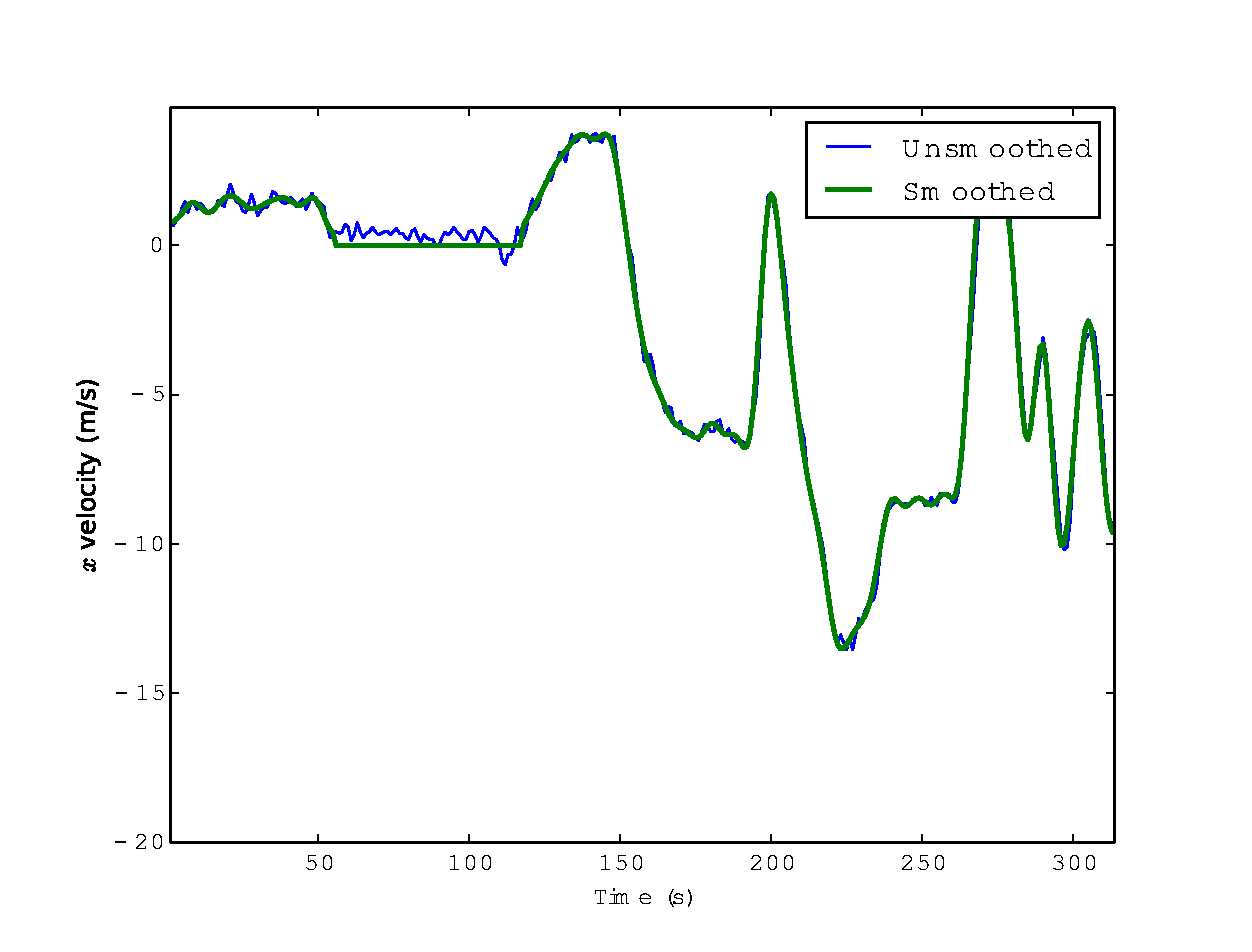
\includegraphics[width=\linewidth]{fouriersmooth}
    \caption{Fourier smoothed velocity component}
    \label{fig:fouriersmooth}
\end{figure}

Another approach attempted was to apply the Savitzky-Golay filter to smooth the data. Savitzky-Golay smooths data by convolution, fitting a polynomial to successive windows over the data points using a least squares optimisation. One can see that in figure \ref{fig:savgolsmooth} that the problem of threshold smoothing is does not appear and that the data appears to be much smoother. However some jaggedness remains in periods of low velocity.

\begin{figure}[h]
    \center
    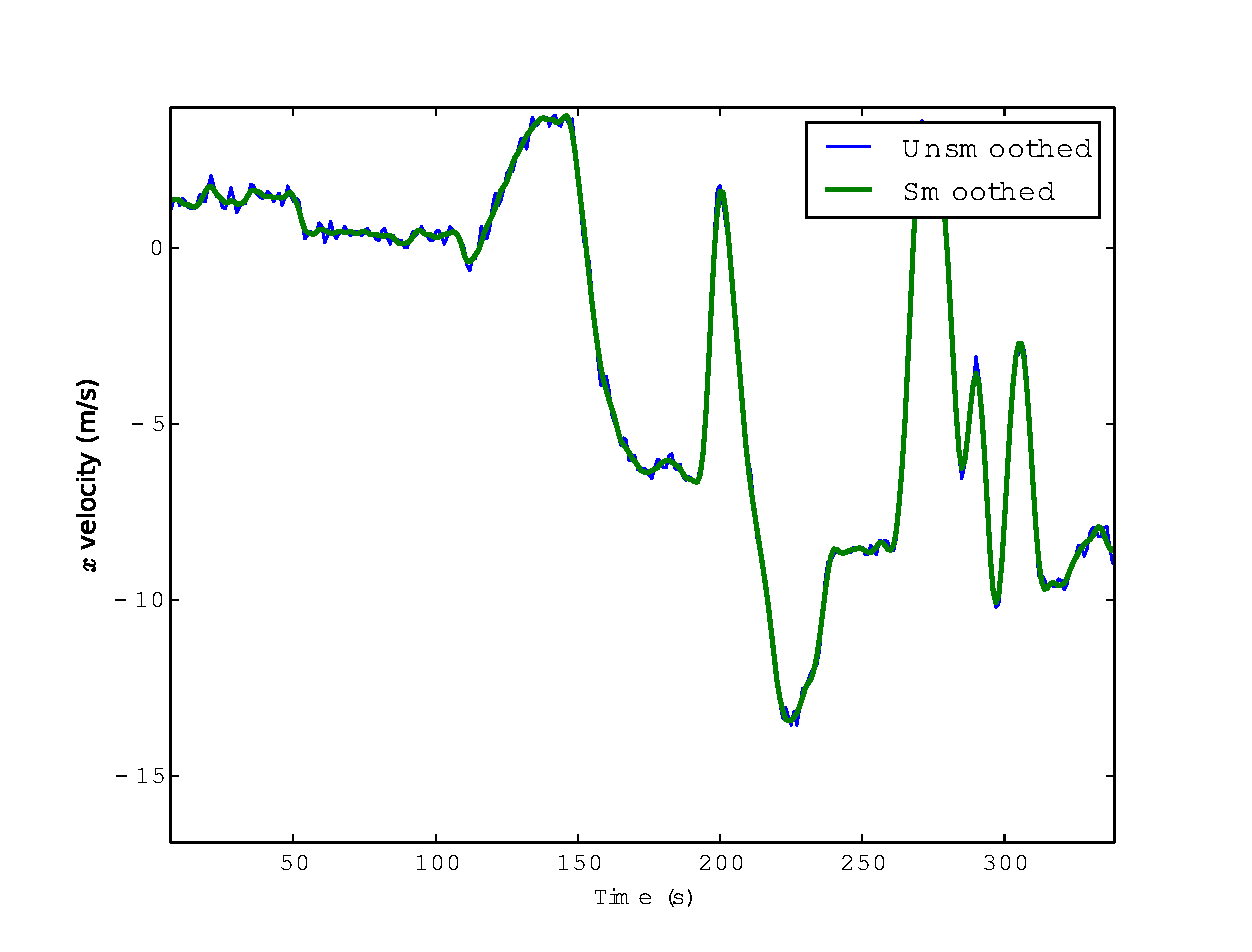
\includegraphics[width=\linewidth]{savgolsmooth}
    \caption{Savitzky-Golay smoothed velocity component}
    \label{fig:savgolsmooth}
\end{figure}


\subsection{Machine Learning}


% put other approaches here

















\subsection{Deep Learning}

While many of the common approaches have demonstrated sufficient performance tackling, machine learning, statistical and prediction-based problems, more recent but advanced methods in the field of \textit{deep learning} have attracted much attention due to their vastly clever architectures and training algorithms. The field started to gain traction when Geoff Hinton \cite{hinton2006fast} released a paper on the discovery of a new training algorithm for deep belief networks.

Deep learning architectures aim to model the structure of the mammal brain, organised in multiple, deep levels \cite{serre2007quantitative}. In the context of image perception, the primary visual cortex serves to extract local features from scenes or images in the form of bars, edges or lines, then build higher level encodings that compute more precise details about the objects being observed \cite{lee1998role}. Deep learning tackles the problem of learning representations using this neurologically inspired mechanism by providing a distributed description of its input in a hierarchical structure of progressively more abstract representations.

A typical deep learning model takes the form of a conventional feedforward neural network with many hidden layers and a deep architecture. However, the term `deep' does not signify the property of a model having many layers but rather the training algorithms used to learn a model in the manner of stacking visible and hidden layers. Depending on the type of architecture, models may be \textit{over-complete} (more hidden nodes than visible nodes), or \textit{under-complete} (more visible nodes than hidden nodes). It has been shown that over-complete representations with appropriate regularisation lead to better performing models \cite{vincent2010stacked}.

To assess the performance of deep learning on our problem, a \textit{Deep Belief Network} (DBN) was trained with the features extracted at the preprocessing stage. A DBN comprises a series of stacked \textit{Restricted Boltzmann Machines} (RBMs). An RBM is a probabilistic graphical model of connected nodes, or more specifically, an energy-based model of variables (or nodes) $\mathbf{x}$ where the energy of the graph is of the form $p(\mathbf{x})=e^{\mathbf{-E(x)}}$, where $\mathbf{E}$ is an energy function. An RBM has two layers -- a visible layer and hidden layer. The objective is to minimise the energy of the model with respect to the weights between the layers. The training algorithm used is called (one-step) \textit{contrastive divergence} \cite{hinton2002training} and works by sampling between the layers so that the hidden layer learns the visible layer at a different dimension while capturing essential information. After training an RBM, another can be stacked on top by using the previous hidden layer as the visible layer for the next RBM.

To build a DBN, three RBMs were trained an `unfolded' into a feedforward neural network with one output node representing the binary decision value of whether a trip belongs to the driver. Each driver was represented by a model specified by the parameters in tables~\ref{table:dbnparams} and~\ref{table:dbnlayers}.

\begin{table}[h]
\centering
\small{
\caption{DBN Parameter Settings}
\label{table:dbnparams}
\begin{tabular}{|l|l|} \hline
\textbf{Parameter}&\textbf{Value}\\ \hline
Activation function & Sigmoid\\ \hline
Batch size & 50\\ \hline
Momentum & 0\\ \hline
Alpha & 1\\ \hline
Training epochs & 5\\ \hline
Model epochs & 50\\ \hline
No. Workers & 16\\ \hline
\end{tabular}}
\end{table}


\begin{table}[h]
\centering
\small{
\caption{DBN Layers}
\label{table:dbnlayers}
\begin{tabular}{|l|l|} \hline
\textbf{Layer}&\textbf{No. nodes}\\ \hline
Input & $N_F$\\ \hline
Hidden & 250\\ \hline
Hidden & 250\\ \hline
Hidden & 250\\ \hline
Output & 1\\ \hline
\end{tabular}}
\end{table}


\subsection{Validation}

\subsection{Large Scale Implementation}





% section
\section{Conclusion}

\subsection{Further Work}


\printbibliography
\end{document}